%!TEX root = ../main.tex

\section{TensorFlow 实战}
\begin{frame}{\secname}
\vfill\hspace{20pt}
\begin{minipage}[m]{0.25\textwidth}
  \linespread{1}\large
  \tableofcontents[sectionstyle = hide/hide, subsectionstyle = show/show/hide]
\end{minipage}%
\hfill%
\begin{minipage}[m]{0.6\textwidth}
  
\includegraphics[height = 7cm]{./icons/programming.pdf}
\end{minipage}%
\vfill
\end{frame}

\subsection{分类问题}
\begin{frame}{\insertsection}{\insertsubsection}
\begin{minipage}[m]{0.48\textwidth}
回到最开始的那个二分类问题, 看看用 \tensorflow{} 是如何解决这个问题的, $500$ 个点的分布如下图所示.

我们通过观察数据的特征, 仍然选用一样的神经网络, 如下图所示.

\centering
\scalebox{0.8}{%
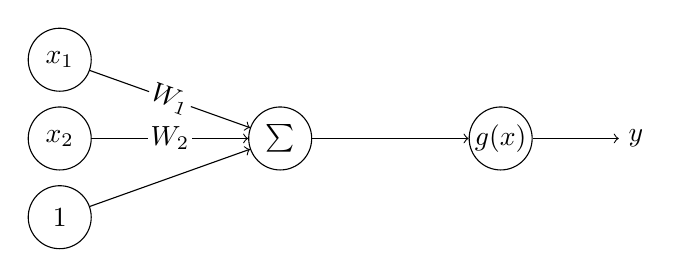
\begin{tikzpicture}[%
  node/.style = {circle, draw, inner sep = 0pt, minimum size = 0.8cm},
  x = 1.4cm]
  \node[node] (x1) at (0, 2) {$x_1$};
  \node[node] (x2) at (0, 1) {$x_2$};
  \node[node] (b)  at (0, 0) {$1$};
  \node[node] (sum) at (2, 1) {$\sum$};
  \node[node] (step) at (4, 1) {$g(x)$};

  \draw[->] (x1) -- (sum) node[midway, fill = white, inner sep = 1pt, sloped] {$W_1$};
  \draw[->] (x2) -- (sum) node[midway, fill = white, inner sep = 1pt, sloped] {$W_2$};
  \draw[->] (b) -- (sum);
  \draw[->] (sum) -- (step);
  \draw[->] (step) -- ++(0:1.5cm) node[anchor = west] {$y$};
\end{tikzpicture}}
\end{minipage}%
\hfill%
\begin{minipage}[m]{0.48\textwidth}
\begin{tikzpicture}
  \begin{axis}[%
    xlabel = $x_1$,
    ylabel = $x_2$,
    height = 7.8cm,
    width = 7cm,
    title = $500$ 个点的分布图
  ]
    \addplot[only marks, discard if not={type}{1}, blue] table[col sep=comma, x = x1, y = x2]{./data/classification/training_data.dat};
    \addplot[only marks, discard if not={type}{0}, green] table[col sep=comma, x = x1, y = x2]{./data/classification/training_data.dat};
  \end{axis}
\end{tikzpicture}
\end{minipage}
\end{frame}

\begin{frame}[fragile]{\insertsection}{\insertsubsection}
这次我们不用计算神经网络的表达式, 直接照着神经网络写 \tensorflow{} 代码即可.

\begin{pythoncode}[fontsize = \fontsize{8}{8}\selectfont]
import tensorflow as tf
import numpy as np

# 定义 $\bm{x} = (x_1, x_2)$, $\bm{W} = (W_1, W_2)$ 和 $b = 1$
x = tf.placeholder(tf.float32, [None, 2])
w = tf.Variable(tf.zeros([2, 1]))
b = tf.constant([1.])

# 定义神经网络输出 $y = g(\bm{W}\bm{x} + 1)$
predict_type = tf.sigmoid((tf.matmul(x, w) + b) * 10)
# 定义真实输出
actual_type = tf.placeholder(tf.float32, [None, 1])
# 定义目标函数 $\ell(\bm{W}) =  -\sum_{i = 1}^{500} y_i\ln g(\bm{W}\bm{x}_i + 1) + (1 - y_i)\ln\big(1 - g(\bm{W}\bm{x}_i + 1)\big)$
loss = -tf.reduce_sum(actual_type * tf.log(predict_type) + (1 - actual_type) * tf.log(1 - predict_type))
\end{pythoncode}

\vspace{-6.3cm}\hfill%
\scalebox{0.8}{%
\begin{tikzpicture}[%
  node/.style = {circle, draw, inner sep = 0pt, minimum size = 0.8cm},
  x = 1.4cm, y = 1.4cm]
  \node[node] (x1) at (0, 2) {$x_1$};
  \node[node] (x2) at (0, 1) {$x_2$};
  \node[node] (b)  at (0, 0) {$1$};
  \node[node] (sum) at (2, 1) {$\sum$};
  \node[node] (step) at (4, 1) {$g(x)$};

  \draw[->] (x1) -- (sum) node[midway, fill = barcolor!5!white, inner sep = 1pt, sloped] {$W_1$};
  \draw[->] (x2) -- (sum) node[midway, fill = barcolor!5!white, inner sep = 1pt, sloped] {$W_2$};
  \draw[->] (b) -- (sum);
  \draw[->] (sum) -- (step);
  \draw[->] (step) -- ++(0:1.5cm) node[anchor = west] {$y$};
\end{tikzpicture}\ \ }
\end{frame}

\begin{frame}[fragile]{\insertsection}{\insertsubsection}
\begin{pythoncode}[fontsize = \fontsize{8}{8}\selectfont]
def load_training_data(path): # 加载训练数据 $\bm{x}$ 和 $\bm{y}$
  with open(path, 'r', encoding = 'utf8') as file:
    next(file)
    lines = [[float(item) for item in line.split()] for line in file]
    xs = np.array([line[:2] for line in lines])
    types = np.array([line[2] for line in lines])[:, None]
  return xs, types

with tf.Session() as session:
  session.run(tf.global_variables_initializer()) # 初始化变量
  train_step = tf.train.GradientDescentOptimizer(0.003).minimize(loss) # 梯度下降法
  xs, types = load_training_data('./training.dat') # 加载训练数据 $\bm{x}$ 和 $\bm{y}$
  for i in range(1000): # 训练 $1000$ 次
    session.run(train_step, feed_dict = {x:xs, actual_type:types}) # 填充训练数据
    # 打印目标函数值
    if i % 10 == 0: print(session.run(loss, feed_dict = {x:xs, actual_type:types}))
  print(session.run(w, feed_dict = {x:xs, actual_type:types})) # 打印最终结果
\end{pythoncode}
\end{frame}

\begin{frame}[fragile]{\insertsection}{\insertsubsection}
最终, 参数 $W_1$ 和 $W_2$ 收敛于点 $(1.07, -3.10)$, 也是非常理想的结果.

\pause
我们还可以换一个目标函数, 用模型预测错误的数量作为目标函数, 其表达式如下所示:
\begin{flalign*}
&& \ell(\bm{W}) &= \sum_{\mathclap{x_1, x_2, y}} \big|H(W_1x_1+ W_2x_2 + 1)) - y\big|\text{,} &&\\
\uncover<3->{\text{由于绝对值不可微,}&& \text{上式} &= \sum_{\mathclap{x_1, x_2, y}} \big(H(W_1x_1+ W_2x_2 + 1)) - y\big)^2\text{,} &&\text{\hphantom{由于绝对值不可微,}}\\}
\uncover<4->{\text{Sigmoid 函数替换,}&& &\approx\sum_{\mathclap{x_1, x_2, y}} \big(g(W_1x_1+ W_2x_2 + 1)) - y\big)^2\text{.} &&}
\end{flalign*}

\uncover<5->{我们修改目标函数的表达式, \uncover<6->{参数 $W_1$ 和 $W_2$ 收敛于点 $(1.07, -3.07)$, 效果拔群.}}\pause\pause\pause
\begin{pythoncode}
loss = tf.reduce_sum(tf.square(actual_type - predict_type))
\end{pythoncode}
\end{frame}

\subsection{拟合问题}
\begin{frame}{\insertsection}{\insertsubsection}
\begin{minipage}[t]{0.41\textwidth}
有 $300$ 个点, 其分布如下图所示, 现在的目标是用一个神经网络, 来拟合这 $300$ 个点.

\begin{center}
\hspace{-10pt}%
\begin{tikzpicture}
\begin{axis}[width = 1.2\textwidth,
             height = 6.4cm]
\addplot[only marks] table[col sep = comma] {./data/fitting/training_data.dat};
\end{axis}
\end{tikzpicture}
\end{center}
\end{minipage}%
\hfill\pause%
\begin{minipage}[t]{0.55\textwidth}
我门用一个两层网络来实现对这些离散点的拟合, 这两层网络的公式为:%
%
\begin{align*}
\bm{x}_2 &= \relu(\bm{W}_1x_1 + \bm{b}_1)\text{,} && \text{$\bm{W}_1\in\mathbb{R}^{10\times1}$, $\bm{b}_1\in\mathbb{R}^{10\times1}$,}\\
\hat{y} &= \bm{W}_2\bm{x}_2 + b_2\text{,}  && \text{$\bm{W}_2\in\mathbb{R}^{1\times10}$, $b_2\in\mathbb{R}^{1\times1}$.}
\end{align*}\pause%
其中, 函数 $\relu(\,\cdot\,)$ 被称为线性整流函数(Rectified Linear Unit, ReLU), 图像如下所示.\vspace{-2pt}

\begin{center}
\hspace{-10pt}%
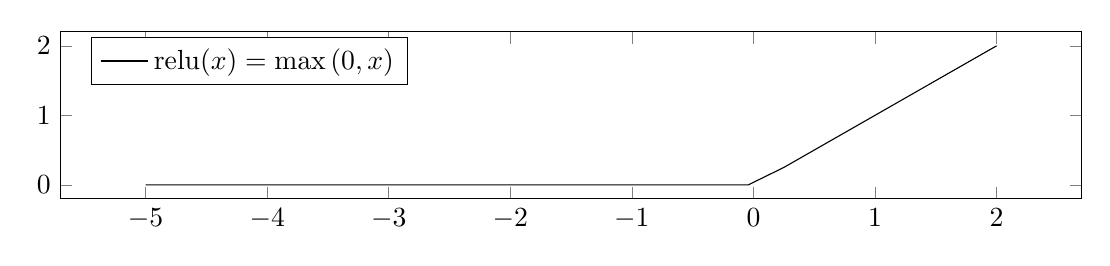
\begin{tikzpicture}
  \begin{axis}[width = 1.2\textwidth,
               height = 3.7cm,
               legend pos = north west,
  ]
    \addplot[mark = none, domain = -5:2] {(x < 0) * 0 + (x >= 0) * x};
    \legend{{$\mathrm{relu}(x) = \max{(0, x)}$}};

  \end{axis}
\end{tikzpicture}
\end{center}
\end{minipage}
\end{frame}

\begin{frame}[fragile]{\insertsection}{\insertsubsection}
\begin{pythoncode}[fontsize = \fontsize{8}{8}\selectfont, escapeinside=||]
import tensorflow as tf
import numpy as np

x1 = tf.placeholder(tf.float32, [None, 1])
w1 = tf.Variable(tf.random_normal([1, 10]))
b1 = tf.Variable(tf.ones([1, 10]))
# $\bm{x}_2 = \relu(\bm{W}_1x_1 + \bm{b}_1)$, $\bm{W}_1\in\mathbb{R}^{10\times1}$, $\bm{b}_1\in\mathbb{R}^{10\times1}$
x2 = tf.nn.relu(tf.matmul(x1, w1) + b1)
w2 = tf.Variable(tf.random_normal([10, 1]))
b2 = tf.Variable(tf.ones([1, 1]))
# $\hat{y} = \bm{W}_2\bm{x}_2 + b_2$, $\bm{W}_2\in\mathbb{R}^{1\times10}$, $b_2\in\mathbb{R}^{1\times1}$
predict_values = tf.matmul(x2, w2) + b2 # 预测值
actual_values = tf.placeholder(tf.float32, [None, 1]) # 真实值

# 目标函数 $\ell(\bm{W}_1, \bm{b}_1, \bm{W}_2, b_2) = \frac{1}{n}\sum_{i = 1}^{300}(y - \hat{y})^2$
loss = tf.reduce_mean(tf.reduce_sum(tf.square(actual_values - |\hspace{50pt}| predict_values), reduction_indices = [1]))
\end{pythoncode}

\vspace{-7.5cm}\hspace{10.5cm}\scalebox{0.53}{\begin{tikzpicture}[%
  tensor/.style = {rectangle, inner sep = 2pt, rounded corners = 0.4cm, draw, align = flush center, minimum height = 0.8cm, minimum width = 0.8cm},
  operator/.style = {tensor, fill = black, draw = none, text = white, inner sep = 2pt},
  line width = 1pt,
  y = 1.1cm
]
\node[tensor, circle]   (x1) at (9, 0) {$\bm{x}_1$};
\node[tensor, circle]   (w1) at (7, 0) {$\bm{W}_1$};
\node[operator]         (t1) at (8, 1) {\mintinline{text}{tf.matmul}};
\node[tensor, circle]   (b1) at (6, 1) {$\bm{b}_1$};
\node[operator]         (p1) at (7, 2) {\mintinline{text}{tf.add}};
\node[operator]         (r1) at (7, 3) {\mintinline{text}{tf.nn.relu}};
\node[tensor, circle]   (w2) at (5, 3) {$\bm{W}_2$};
\node[operator]         (t2) at (6, 4) {\mintinline{text}{tf.matmul}};
\node[tensor, circle]   (b2) at (4, 4) {$b_2$};
\node[operator]         (p2) at (5, 5) {\mintinline{text}{tf.add}};
\node[tensor]           (pv) at (5, 6) {\mintinline{text}{prediction_values}};
\node[tensor]           (av) at (8, 6) {\mintinline{text}{actual_values}};
\node[operator]         (sb) at (6.5, 7.5) {\mintinline{text}{tf.sub}};
\node[operator]         (sq) at (6.5, 8.5) {\mintinline{text}{tf.square}};
\node[operator]         (rs) at (6.5, 9.5) {\mintinline{text}{tf.reduce_sum}};
\node[operator]         (rm) at (6.5, 10.5) {\mintinline{text}{tf.reduce_mean}};
\node[tensor]           (ls) at (6.5, 11.5) {\mintinline{text}{loss}};

\draw[->] (x1) -- (t1);
\draw[->] (w1) -- (t1);
\draw[->] (b1) -- (p1);
\draw[->] (t1) -- (p1);
\draw[->] (p1) -- (r1);
\draw[->] (w2) -- (t2);
\draw[->] (r1) -- (t2);
\draw[->] (b2) -- (p2);
\draw[->] (t2) -- (p2);
\draw[->] (p2) -- (pv);
\draw[->] (pv) -- (sb);
\draw[->] (av) -- (sb);
\draw[->] (sb) -- (sq);
\draw[->] (sq) -- (rs);
\draw[->] (rs) -- (rm);
\draw[->] (rm) -- (ls);
\end{tikzpicture}}
\end{frame}

\begin{frame}[fragile]{\insertsection}{\insertsubsection}
\begin{pythoncode}[fontsize = \fontsize{8}{8}\selectfont]
def load_training_data(path): # 读取训练数据
    with open(path, 'r', encoding = 'utf8') as file:
        next(file)
        lines = [[float(item) for item in line.split(',')] for line in file]
    return (np.array([line[i] for line in lines])[:, None] for i in [0, 1])

with tf.Session() as session: # 初始化 Session
  session.run(tf.global_variables_initializer()) # 初始化变量

  (input_data, output_data) = load_training_data('./training_data.dat') # 加载训练数据
  train_step = tf.train.GradientDescentOptimizer(0.1).minimize(loss) # 设置目标函数

  for i in range(1000): # 训练 $1000$ 次
    session.run(train_step, feed_dict = {x1:input_data, actual_values:output_data})
    if i % 50 == 0:
      print(session.run(loss, feed_dict = {x1:input_data, actual_values:output_data}))
\end{pythoncode}
\end{frame}

\begin{frame}{\insertsection}{\insertsubsection}
训练 $1000$ 次后, 目标函数 $\ell(\bm{W}_1, \bm{b}_1, \bm{W}_2, b_2) = 2.48\times 10^{-3}$, 此时拟合函数的图像如图所示.\vspace{10pt}

\begin{tikzpicture}
\begin{axis}[width = 1\textwidth,
             height = 6.4cm,
             xlabel = $x$,
             ylabel = $y$,
             title = 训练数据与拟合曲线,
             legend pos = south east]
\addplot[only marks] table[col sep = comma] {./data/fitting/training_data.dat};
\addplot[mark = none,white, line width = 1pt, double = red, double distance = 2pt, on layer = foreground] table[col sep = comma, x = x, y = y] {./data/fitting/fitting_line.dat};
\legend{训练数据, 拟合曲线}
\end{axis}
\end{tikzpicture}
\end{frame}

\subsection{调试}
\begin{frame}[fragile]{\insertsection}{\insertsubsection-TensorBoard}
可以用 TensorBoard 来可视化 \tensorflow{} 的训练过程, 帮助用户了解训练过程。启动 TensorBoard 首选需要记录训练过程数据:

\begin{pythoncode}[fontsize = \fontsize{8}{8}\selectfont]
# 建立数据流图 ...
tf.summary.histogram('w2', w2) # 需要记录 $\bm{W}_2$
tf.summary.scalar('loss', loss) # 需要记录目标函数 $\ell$
merged = tf.summary.merge_all() # 合并需要记录的数据
with tf.Session() as session:
  writer = tf.summary.FileWriter('./tensorboard/') # 新建一个记录器
  writer.add_graph(session.graph) # 关联会话中的数据流图
  # 其他初始化 ...
  for i in range(1000):
    # 训练网络 ...
    writer.add_summary(session.run(merged, feed_dict = {x1:input_data, actual_values:output_data}), i)
    # 其他操作 ...
\end{pythoncode}
\end{frame}

\begin{frame}[fragile]{\insertsection}{\insertsubsection-TensorBoard}
然后在终端中运行如下代码来启动 TensorBoard.
\begin{shellcode}[fontsize = \fontsize{8}{8}\selectfont]
tensorboard --logdir=tensorboard
\end{shellcode}
\pause

\vspace{-5pt}%
有时候系统会提示 \inlinetext{command not found: tensorboard}, 此时需要找到 TensorBorad 在哪. 首选在 Python 的终端中运行如下脚本, 获得 TensorBoard 的路径.%
\begin{pythoncode}[fontsize = \fontsize{8}{8}\selectfont]
>>> import tensorboard
>>> print(tensorboard.__file__)
/path/of/your/tensorboard/__init__.py # $\leftarrow$ 这个就是路径
\end{pythoncode}
\pause

\vspace{-5pt}%
然后在系统终端运行如下脚本即可启动 TensorBoard. 查看当前训练的 TensorBoard, 可以用浏览器访问 \inlinetext{http://127.0.0.1:6006/} 这个地址.
\begin{shellcode}[fontsize = \fontsize{8}{8}\selectfont]
python /path/of/your/tensorboard/|\texttt{\textcolor{red}{main}}|.py --logdir=tensorboard
\end{shellcode}
\end{frame}

\begin{frame}[fragile]{\insertsection}{\insertsubsection-tfdbg}
\begin{quote}
\tensorflow{} 中使用 Python 描述计算图, 再使用 C++ 后端进行训练时就非常不容跟踪调试, \tensorflow{} 提供了 tfdbg 模块用于解决这个问题.

\hfill from: \href{https://jiexiao111.github.io/2017/10/17/Tensorflow-tfdbg.html}{JieXiao's Blog --- 《\tensorflow{} tfdbg》}
\end{quote}

\pause
启动 tfdbg 很容易, 只要在原始的代码中添加两行代码即可, 再次运行便会进入 tfdbg 界面, 在这里可以插入断点, 单步运行 \tensorflow{} 的训练过程, 查看每一个张量的值.
\begin{pythoncode}[fontsize = \fontsize{8}{8}\selectfont]
import tensorflow as tf
from tensorflow.python import debug as tf_debug # 第一行代码加在这
# 建立数据流图 ...
with tf.Session() as session:
  sess = tf_debug.LocalCLIDebugWrapperSession(sess) # 第二行代码加在这
  # 初始化 ...
  # 训练模型 ...
\end{pythoncode}

\end{frame}


% \begin{frame}[fragile]{\insertsection}{\insertsubsection}
% 我门用一个两层网络来实现对这些离散点的拟合, 这两层网络的公式为:%
% %
% \begin{flalign*}
%   && x_2 &= \relu(W_1x_1 + b_1)\text{,} && \text{$W_1\in\mathbb{R}^{10\times1}$, $b_1\in\mathbb{R}^{10\times1}$,} &&\\
%   && \hat{y} &= W_2x_2 + b_2\text{,}                  && \text{$W_2\in\mathbb{R}^{1\times10}$, $b_2\in\mathbb{R}^{1\times1}$.} &&
% \end{flalign*}

% \begin{minipage}[m]{0.38\textwidth}
% \begin{tikzpicture}
%   \begin{axis}[width = 1.2\textwidth,
%                height = 5.1cm,
%                legend pos = north west,
%   ]
%     \addplot[mark = none, domain = -2:5] {(x < 0) * 0 + (x >= 0) * x};
%     \legend{{$\mathrm{relu}(x) = \max{(0, x)}$}};

%   \end{axis}
% \end{tikzpicture}
% \end{minipage}%
% \hfill%
% \begin{minipage}[m]{0.60\textwidth}
% \begin{pythoncode}
% x1 = tf.placeholder(tf.float32, [None, 1])
% w1 = tf.Variable(tf.random_normal([1, 10]))
% b1 = tf.Variable(tf.ones([1, 10]))

% x2 = tf.nn.relu(tf.matmul(x1, w1) + b1)
% w2 = tf.Variable(tf.random_normal([10, 1]))
% b2 = tf.Variable(tf.ones([1, 1]))
% y = tf.matmul(x2, w2) + b2
% \end{pythoncode}
% \end{minipage}
% \end{frame}

% \subsection{训练网络}
% \begin{frame}[fragile]{\insertsection}{\insertsubsection}
% 我们用统计学中的均方误差作为代价函数来训练网络, 如下所示.%
% %
% \[
%   \ell(W_1, b_1, W_2, b_2) = \frac{1}{n}\sum_{i = 1}^n (y - \hat{y})^2\text{.}
% \]%
% %
% 根据上式可以写出 TensorFlow 中的训练目标.
% \begin{pythoncode}
% actual_values = tf.placeholder(tf.float32, [None, 1])
% loss = tf.reduce_mean(tf.reduce_sum(tf.square(actual_values - y), reduction_indices = [1]))

% train_step = tf.train.GradientDescentOptimizer(0.1).minimize(loss)
% \end{pythoncode}

% 我们可以看出, \inlinepython{tf.placeholder} 一般对应着训练数据, 因为训练数据只能在训练的时候给出, 在定义计算图的时候不知道具体的值, \inlinepython{tf.placeholder} 起占位的作用.
% \end{frame}

% \begin{frame}[fragile]{\insertsection}{\insertsubsection}
% 训练网络的过程, 就是求使代价函数 $\ell(W_1, b_1, W_2, b_2)$ 达到最小值时的参数集合 $W_1$, $b_1$, $W_2$, $b_2$. 而且需要启动一个会话 \inlinepython{tf.Session} 来完成运算图的计算.

% \begin{pythoncode}
% session = tf.Session()
% session.run(tf.initialize_all_variables())

% for step in range(1000):
%     feed_dict = {x1:input_data, actual_values:output_data}
%     session.run(train_step, feed_dict = feed_dict)

%     if step % 50 == 0:
%         print(session.run(loss, feed_dict = feed_dict))

% session.close()
% \end{pythoncode}
% \end{frame}

% \subsection{测试网络}

% \subsection{}